\section{Closedness of the density restriction}
\label{sec:splitting}

\begin{proof}[Proof of Theorem~\ref{thm:splitting}]
The existence of the density is Lemma~\ref{lem:density}.
We approximate the positive-density restriction by smooth
functions of a regularized density. Closedness of \(T\) then
reduces the problem to controlling full derivatives against
\(Q\) and tangential derivatives against \(P\). The tangential
estimate combines the quantitative angular bound with the
vanishing transverse moment from Lemma~\ref{lem:transverse};
their product will make the cutoff boundary tend to zero.
Choose a nonnegative, smooth, nonincreasing function
\(h:[0,\infty)\to[0,\infty)\), positive near zero and zero
on a neighborhood of \([1,\infty)\). For \(r\) below the
injectivity radius define
\begin{equation}\label{eq:density-cutoff}
f_r(x)=r^{-2}\int_Xh(d_g(x,y)^2/r^2)\dd\mu(y).
\end{equation}
The kernel is smooth near the diagonal and vanishes before
the cut locus, so \(f_r\) is smooth. It is uniformly bounded.
Writing \(H(t)=h(t^2)\), integration of ball indicators gives
\[
f_r(x)=\int_0^1[-H'(t)]r^{-2}\mu(B_{rt}(x))\dd t
 \longrightarrow c_h\theta(x),
\qquad
c_h=\int_0^1h(u)\dd u>0.
\]
The quadratic growth bound supplies domination for this
limit. In particular \(\theta\) is Borel measurable.
Differentiation of the finite measure \(\mu\) with respect
to four-dimensional volume also shows that
\begin{equation}\label{eq:theta-volume}
\theta(x)=0\quad\text{for volume-almost every }x.
\end{equation}
Indeed, apply the differentiation theorem for Radon measures
\cite[Theorem~4.19]{Kinnunen2026} in a fixed coordinate chart,
with smooth volume as the denominator measure. At
volume-almost every center the measure-to-volume ratios
of sufficiently small coordinate balls are bounded.
Enclosing a geodesic ball of radius \(r\) in a coordinate
ball of comparable radius therefore gives
\(\mu(B_r(x))=O_x(r^4)\), and hence
\(r^{-2}\mu(B_r(x))\to0\).

\subsection*{The error from the \(L^2\) correction}

Put \(M_r(x)=\mu(B_r(x))\). Cauchy--Schwarz gives
\begin{align}
r^{-3}\int_X|Q|M_r\vol
&\le
\left(\int_X|Q|^2r^{-2}M_r\vol\right)^{1/2}
\left(\int_Xr^{-4}M_r\vol\right)^{1/2}
\longrightarrow0.
\label{eq:q-cutoff}
\end{align}
For the second factor, Fubini and the four-dimensional
volume bound give
\[
\int_Xr^{-4}M_r(x)\,dV_g(x)
=r^{-4}\int_X\operatorname{vol}_g(B_r(y))\dd\mu(y)
\le C\mu(X).
\]
For the first, \(r^{-2}M_r\) is bounded and tends to zero
volume-almost everywhere by \eqref{eq:theta-volume}.
Dominated convergence applies to \(|Q|^2\).

First variation gives \(|df_r(x)|\le Cr^{-3}M_r(x)\).
Thus \eqref{eq:q-cutoff} also proves
\begin{equation}\label{eq:q-full-derivative}
\int_X|Q|\,|df_r|\vol\longrightarrow0.
\end{equation}

\subsection*{Tangential derivatives of the density cutoff}

We prove the complementary estimate
\begin{equation}\label{eq:tangential-cutoff}
\int_{\mathscr C}|df_r(x)|_{L_\ell}\dd\lambda(x,\ell)
\longrightarrow0,
\end{equation}
where the subscript means restriction of the covector to
the two-plane \(L_\ell\).

For \((x,\ell)\in\mathscr C\), \(y\in B_r(x)\), and
\(m\in\mathscr C_y\), put
\[
z=z_x(y),\qquad z^\perp=\pr_{L_\ell^\perp}z,
\qquad \delta=|\ell-\tau_{yx}m|.
\]
These quantities measure different errors
(Figure~\ref{fig:cutoff-geometry}). Closedness will replace a
derivative along \(L_\ell\) by normal derivatives. Differentiating
the radial kernel normally contributes \(|z^\perp|/r\), while
the resulting mixed two-forms contribute \(\delta\).
Keeping these factors together is what makes their integrated
product overcome the cutoff's \(r^{-3}\) normalization.

\begin{figure}[tb]
\centering
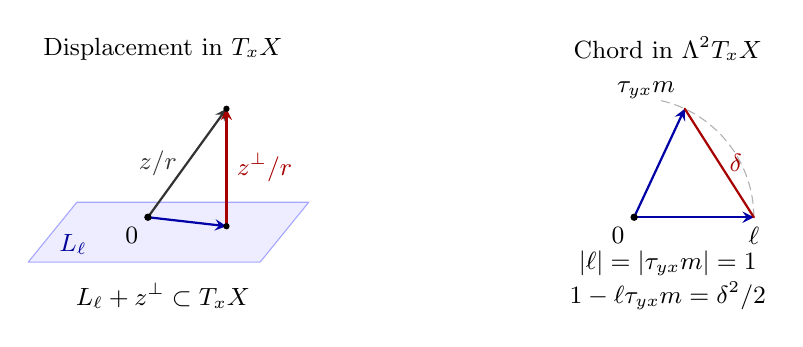
\begin{tikzpicture}[>=stealth, line cap=round, line join=round,
                    font=\small, scale=0.95]
  \begin{scope}
    \node at (0.2,2.25) {Displacement in \(T_xX\)};
    \filldraw[fill=blue!7, draw=blue!35]
      (-1.6,-0.6) -- (1.5,-0.6) -- (2.15,0.2) -- (-0.95,0.2) -- cycle;
    \node[blue!60!black] at (-1.0,-0.37) {\(L_\ell\)};
    \coordinate (O) at (0,0);
    \coordinate (Zt) at (1.05,-0.12);
    \coordinate (Z) at (1.05,1.45);
    \draw[->,thick,blue!65!black] (O) -- (Zt);
    \draw[->,thick,black!80] (O) -- (Z)
      node[midway,left] {\(z/r\)};
    \draw[->,thick,red!65!black] (Zt) -- (Z)
      node[midway,right] {\(z^\perp/r\)};
    \fill (O) circle (1.4pt);
    \node[below left] at (O) {\(0\)};
    \fill (Zt) circle (1.2pt);
    \fill (Z) circle (1.2pt);
    \node at (0.2,-1.05) {\(L_\ell+\R z^\perp\subset T_xX\)};
  \end{scope}
  \begin{scope}[xshift=6.5cm]
    \node at (0.45,2.25) {Chord in \(\Lambda^2T_xX\)};
    \coordinate (O) at (0,0);
    \coordinate (A) at (1.6,0);
    \coordinate (B) at (65:1.6);
    \draw[densely dashed,black!30] (1.6,0) arc (0:78:1.6);
    \draw[->,thick,blue!65!black] (O) -- (A);
    \draw[->,thick,blue!65!black] (O) -- (B);
    \draw[thick,red!65!black] (A) -- (B)
      node[midway,right] {\(\delta\)};
    \node[below] at (A) {\(\ell\)};
    \node[above left] at (B) {\(\tau_{yx}m\)};
    \fill (O) circle (1.4pt);
    \node[below left] at (O) {\(0\)};
    \node at (0.45,-0.62) {\(|\ell|=|\tau_{yx}m|=1\)};
    \node at (0.45,-1.05) {\(1-\ip{\ell}{\tau_{yx}m}=\delta^2/2\)};
  \end{scope}
\end{tikzpicture}
\caption{The two factors in the tangential cutoff estimate.
The left panel lies in the subspace spanned by \(L_\ell\) and
the normal displacement. The right panel lies in the span of
two unit bivectors, in a different ambient vector space.
Closedness produces the product \(\delta|z^\perp|/r\).
The squared integrals of its factors are \(\ang_r=O(r^4)\)
and \(\trans_r=o(r^2)\), respectively.}
\label{fig:cutoff-geometry}
\end{figure}

Fix \((x,\ell)\). Choose orthonormal normal coordinates
\(z=z_x(y)\) with \(\ell=e_1\wedge e_2\), and put
\(h_r(z)=h(|z|^2/r^2)\).
At the fixed center \(x\), first variation of squared
distance gives
\(d_x[d_g(x,y)^2](e_i)=-2z_i\). Hence, for \(i=1,2\),
\begin{equation}\label{eq:center-derivative}
df_r(x)e_i=-r^{-2}\int_X\partial_{z_i}h_r\dd\mu(y).
\end{equation}
This differentiates the scalar distance kernel. We now
freeze \(x,\ell\), and these coordinates, and use closedness
of \(T\) in the \(y\) variable.

Coordinate covectors in normal coordinates differ from
radially parallel covectors by \(O(|z|^2)\). Indeed, the
Jacobi equation along \(t\mapsto\exp_x(tz)\), in a parallel
frame, has curvature coefficient \(O(|z|^2)\). The field
with initial data \((0,v)\) is therefore
\(tv+O(|z|^2|v|)\) for \(0\le t\le1\), giving
\(\tau_{yx}\circ d(\exp_x)_z=\Id+O(|z|^2)\).
Inverting gives the same estimate for coordinate covectors.
Since both line bivectors have norm one,
\begin{equation}\label{eq:quadratic-coordinate}
(dz_1\wedge dz_2)(m)
=\ip{\ell}{\tau_{yx}m}+O(r^2)
=1-\tfrac12\delta^2+O(r^2)\qquad(|z|<r).
\end{equation}
All errors are uniform. Comparing
\eqref{eq:center-derivative} with the \(P\) part of the
current below, and bounding its \(Q\) part, gives
\begin{align}
\left|df_r(x)e_i+
r^{-2}T\bigl((\partial_{z_i}h_r)\,dz_1\wedge dz_2\bigr)\right|
&\le Cr^{-3}\int_{d_g(x,y)<r}(\delta^2+r^2)
                    \dd\lambda(y,m)\nonumber\\
&\quad+Cr^{-3}\int_{B_r(x)}|Q|\vol.
\label{eq:comparison-error}
\end{align}
After integration against \(\lambda(x,\ell)\), its first
term is \(O(r)\) by \eqref{eq:abstract-angular}. Its
\(r^2\) term is \(O(r)\) by \eqref{eq:abstract-growth}.
Its last term tends to zero by Fubini and
\eqref{eq:q-cutoff}. Thus the integrated comparison error
vanishes.

For \(i=1\), apply closure to \(d(h_rdz_2)\); for \(i=2\),
apply it to \(d(h_rdz_1)\). These one-forms are compactly
supported in the chart and extend smoothly by zero.
Since \(d(dz_j)=0\), each
\(T\bigl((\partial_{z_i}h_r)\,dz_1\wedge dz_2\bigr)\)
is, up to sign, a sum of terms
\[
T\bigl((\partial_{z_a}h_r)\,dz_a\wedge dz_j\bigr),
\qquad a=3,4,\quad j\in\{1,2\}.
\]
For the normal derivatives,
\[
|\partial_{z_a}h_r|
\le Cr^{-1}\left|\pr_{L_\ell^\perp}(z/r)\right|.
\]
The mixed coordinate two-forms satisfy
\[
|(dz_a\wedge dz_j)(m)|\le C(\delta+r^2).
\]
Indeed their radially parallel counterparts vanish on
\(\ell\), and their coordinate error is \(O(r^2)\).

The integrated \(Q\) and \(r^2\) errors are controlled as
in \eqref{eq:comparison-error}. Including the outer factor
\(r^{-2}\), the remaining term is at most
\[
Cr^{-3}\iint_{d_g(x,y)<r}
\delta\left|\pr_{L_\ell^\perp}(z_x(y)/r)\right|
\dd\lambda(y,m)\dd\lambda(x,\ell).
\]
By Cauchy--Schwarz, \eqref{eq:abstract-angular}, and
Lemma~\ref{lem:transverse}, this is bounded by
\begin{equation}\label{eq:critical-scaling}
Cr^{-3}\sqrt{\ang_r}\sqrt{\trans_r}
=r^{-3}O(r^2)o(r)=o(1).
\end{equation}
The second squared integral is exactly \(\trans_r\),
since its integrand does not depend on \(m\).
Combining with \eqref{eq:comparison-error} proves
\eqref{eq:tangential-cutoff}. No derivative of a
center-dependent frame occurs: first variation was
applied before the fixed-chart current tests.

\subsection*{Passing to the positive-density set}

Let \(b:\R\to\R\) be smooth with \(b(0)=0\).
On the uniformly bounded range of \(f_r\), both \(b\)
and \(b'\) are bounded. Dominated convergence gives
\begin{equation}\label{eq:weighted-current-limit}
b(f_r)T\longrightarrow b(c_h\theta)P
\end{equation}
as currents. For \(P\) this follows from pointwise
convergence of \(f_r\). For \(Q\) it follows from
\eqref{eq:theta-volume} and \(Q\in L^1\).

If \(\eta\) is a smooth one-form, closedness of \(T\)
and the product rule give
\[
(b(f_r)T)(d\eta)
=-T\bigl(b'(f_r)\,df_r\wedge\eta\bigr).
\]
The \(Q\) contribution tends to zero by
\eqref{eq:q-full-derivative}. A line bivector \(\ell\)
evaluates \(df_r\wedge\eta\) using only the restriction
of \(df_r\) to \(L_\ell\), so the \(P\) contribution
tends to zero by \eqref{eq:tangential-cutoff}.
It follows from \eqref{eq:weighted-current-limit} that
\(b(c_h\theta)P\) is closed.

Finally take \(b_n(s)=1-e^{-ns}\). On the relevant
nonnegative range, \(0\le b_n\le1\) and
\(b_n(c_h\theta)\to\ind_E\).
A second dominated-convergence limit proves that
\(P_E=\ind_EP\) is closed. The limits are successive:
first \(r\downarrow0\) for each fixed \(n\), then
\(n\to\infty\). No bound on \(b_n'\) uniform in \(n\)
is required.
\end{proof}
